%!TeX root=../../main.tex
\chapter{Introduction}                                 \label{ch:introduction}
\section{Context}  \label{sec:context}
Application software is everywhere: ranging from social media apps to online web shops, login systems, healthcare systems and even Photoshop. The usage of these applications is irreversibly integrated with our way of living, powered by wireless internet connections, personal computers, mobile devices and many more technologies to access them whenever and wherever we want. It comes as no surprise that the demands of these systems have therefore increased over time which in turn introduced entire new ranges of problems. One of these problems is how to cost-effectively scale the computational resources to handle a fluctuating amount of end-users. For example, a web shop might have 20 times more clients during December due to the holiday season than any other month of the year, and as a result, the servers are not being used to their capacity for 11 months a year.
\\[10pt]

 One of the solutions to handle this increased and fluctuating demand is the trend towards cloud native computing: the practice of building and running dynamically scaling applications in cloud environments \cite{CNCF}. This is not unexpected, since cloud native computing offers advantages such as scalability, resource efficiency and security \cite{cnci4}. Although cloud native computing is not a new phenomenon it seems to only grow in popularity \cite{CNCFSurvey} and is rapidly replacing old legacy systems and in-house servers. One of the key components to enable this growth are container formats built upon the specifications of the Open Container Initiative \acrshort{oci} \cite{OCI}, such as Containerd. These containers are a source of application portability by including the application code and all the dependencies required to run the code. This means they can easily be run in any environment by container engines like rkt \cite{rkt}, CRI-O \cite{crio}, LXC \cite{LXC} and Docker \cite{Bernstein2014}. Benefits of these containers include. but are not limited to, the possibility of easily changing geographic location to ensure faster user connections and having multiple deployments of the same container to serve more users by spreading the workload. 
\\[10pt]

 However, new problems arise when demand increases and clusters of sometimes even thousands of containerised applications need to be created to meet those demands. This is where orchestration solutions such as Kubernetes (\acrshort{k8s}) \cite{Bernstein2014} and Mesos \cite{Mesos} come into play. They allow automatic handling of deployment, load balancing of users, scaling of resources and containers, defining security practices and monitoring of the applications, all based on settings defined by the cluster manager.
\\[10pt]

\acrshort{k8s} is currently the standard container orchestration tool in the cloud community according to the 2022 Cloud Native Computing Foundation annual survey, as seen in the data excerpt shown in \autoref{tab:k8susage} \cite{CNCFSurvey}. A Kubernetes cluster consists of many different components such as nodes, which are the highest-level component that run on physical or virtual machines and are responsible for either managing the cluster, running one or more pods, or both. Pods are the lowest-level component in Kubernetes and specify how one or more containerised applications should be run. Pods give their containerised applications access to networking resources and shared storage and allow for duplication of these containerised applications to increase workload. To ensure the security of clusters Kubernetes has different solutions for different attack surfaces. One of these solutions is the network policies that define rules for traffic flow between pods. These network policies work based on key-value labels to select the pods they are applied to and are intended to restrict communication between pods to counter network congestion and the spread of malicious attacks from compromised pods \cite{nps}.
\\[10pt]
\begin{table}[h]
    \centering
    \begin{tabular}{|c|c|c|}
        \hline
        \textbf{User Type} & \textbf{Using \acrshort{k8s} in Production (\%)} & \textbf{Using \acrshort{k8s} in Piloting/Evaluating (\%)} \\
        \hline
        End Users & 64 & 25 \\
        Non-End Users & 49 & 20 \\
        \hline
    \end{tabular}
    \caption{Kubernetes Usage Data \cite{CNCFSurvey}}
    \label{tab:k8susage}
\end{table}
\begin{quote}
\textit{"CNCF End Users are member companies that utilize cloud native technologies internally, refrain from selling any cloud-native services externally, and do not fall under the categories of vendors, consultancies, training partners, or telecommunications companies. Individuals within these end user companies are passionate about solving problems using cloud native architectures and providing teams with self-service solutions which create a more inclusive, iterative process." \cite{CNCFSurvey}}
\end{quote}

In order to work, the Kubernetes nodes need to be deployed on servers or virtual machines that offer correct networking interfaces and computational resources. OpenStack allows us to easily orchestrate these \acrshort{vm}s while offering automation of these aforementioned functionalities along with the possibility to add functionalities according to the needs of the cluster. One of these functionalities is the security groups and security group rules, which select \acrshort{vm} instances based on assigned security groups or IP addresses to restrict communication between instances \cite{sg} \cite{sgrule}. the goal of the security group rules is comparable to that of the Kubernetes network policies, although they work on a lower level in the technology stack to achieve it. Balancing between restricting communication while still allowing the minimum required connections for correct execution of the virtual machines is a daunting task, and is not necessarily made easier by the dynamic natures of instances and the Kubernetes nodes.


% ===============================================================
\section{Problem} \label{sec:problem}
\acrlong{k8s} talks about the 4 C’s of cloud-native security on their website as seen in \autoref{fig:4cs}: The code, container, cluster and cloud layer \cite{4cs}. The code and container layer can be secured with defensive programming guidelines \cite{defensiveprogramming} and specifications such as those of \acrshort{oci} \cite{OCI}. However, they cannot safeguard against misconfiguration of the cluster and cloud layer. Imagine a container on the cluster being compromised by a malicious attacker. In the worst case, this scenario can lead to an entire cluster of infected pods and containers due to unrestricted communication. Luckily there are security principles available such as network policies in \acrshort{k8s} and security groups in Openstack that can try to mitigate these risks. These two examples are present in the cluster and cloud layer respectively \cite{nps} \cite{secgroups}.
\\[10pt]

\begin{figure}[htbp]
  \centering
  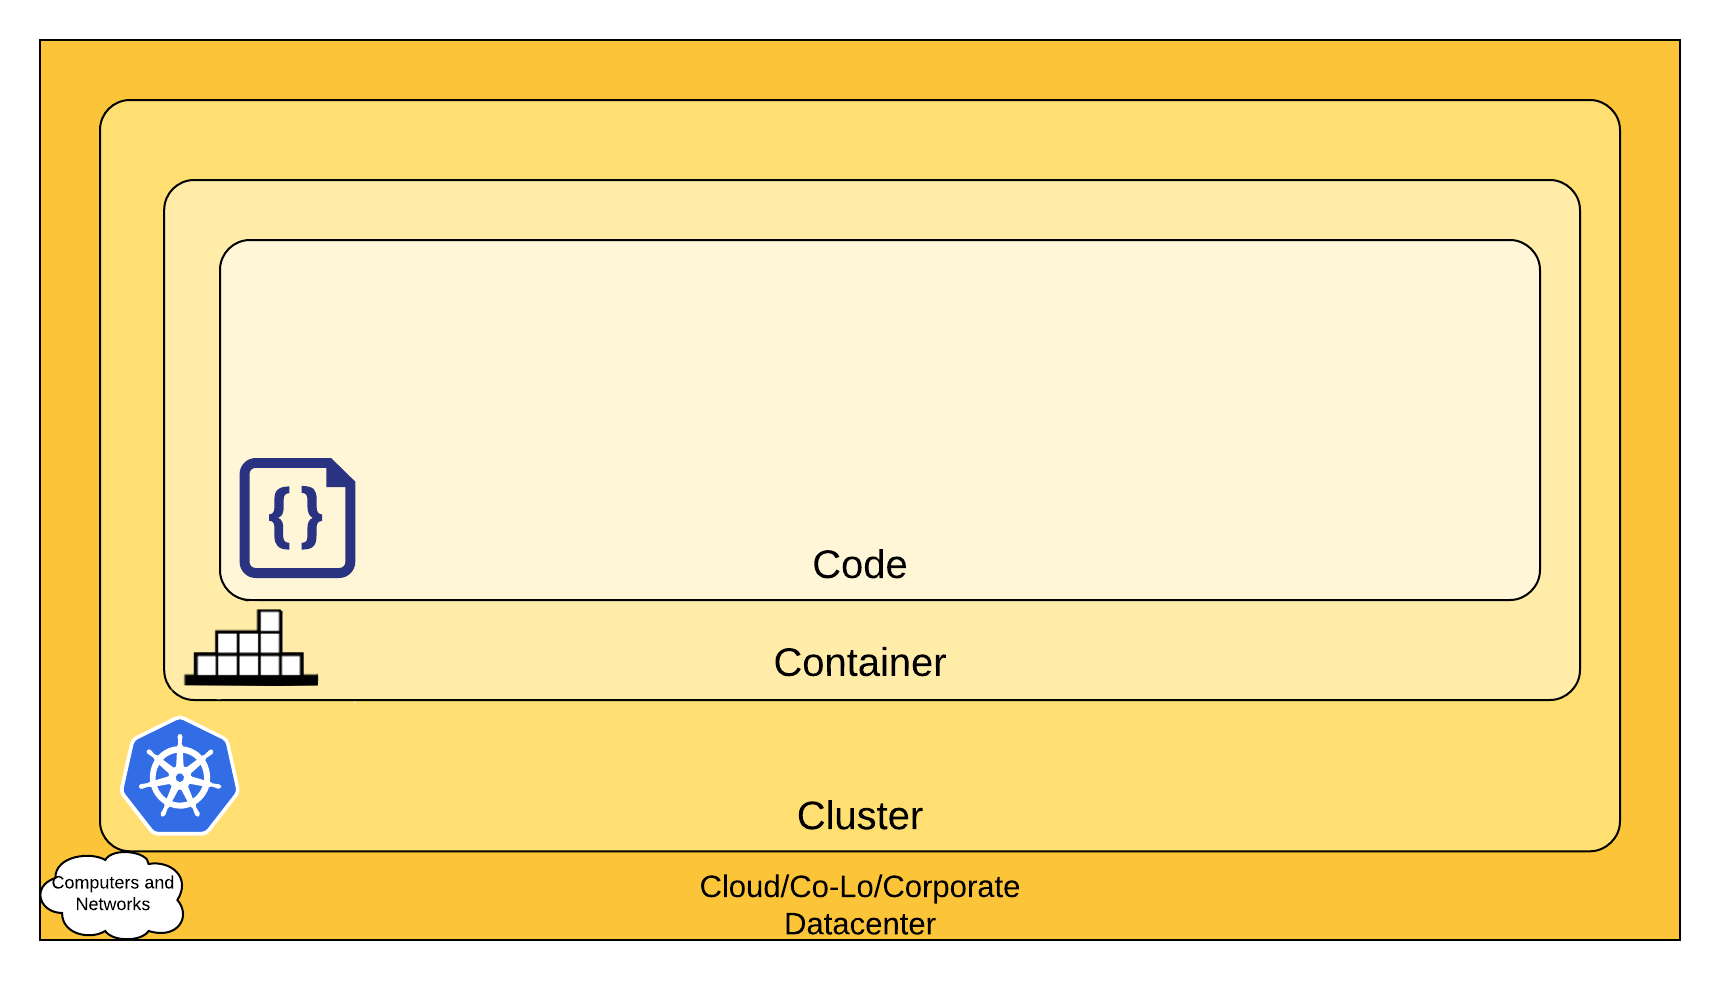
\includegraphics[width=0.8\textwidth]{images/4c.png}
  \caption{The 4C's of Cloud Native security (taken from source \cite{4cs})}
  \label{fig:4cs}
\end{figure}

Although the configuration of the Kubernetes network policies and their intended effect might remain consistent, their result might deviate from the expectations due to changes in the cluster state. Kubernetes pods might be added, updated or removed and depending on the matches between its applied labels and existing \acrshort{np} label selectors this can result in unwanted or missing connections. Even when such unwanted network behaviour gets caught it might be hard to resolve due to the size of the cluster. The scale of this problem increases when we take into account that this same issue can happen when adding, updating or removing Kubernetes network policies or OpenStack security groups and security group rules. Additionally, these different configurations in the separate layers of the 4C's security model can negatively impact each other. We will illustrate this impact with an example.
\\[10pt]

Imagine a cluster with two deployed containers: a web application and a database upon which the web application depends for the data that will need to be displayed. The application manager responsible for the web application knows of this dependency on the database and defines the correct network policies in the cluster layer so that the containers can communicate. What the application manager does not know however is that the person responsible for the \acrshort{vm}s in the cloud layer, who we will call the cloud manager, works according to the principle of least-privilege \cite{leastprivilige}. As a result, the \acrshort{vm}s on which the containers are deployed are prevented from communicating by their networking rules, since they had no reason to communicate before the deployments. We now have a conflict between the cluster and cloud layer which results in an unreachable database container and a non-functioning web application.
\\[10pt]

These types of conflict can easily be overlooked and need to be verified often due to the constantly changing state of a cluster. Additionally, keeping the principle of least privilege enforced while allowing necessary communication gets more complicated as the size of the cluster grows as well. At the moment of writing and to the best of our knowledge there is currently no solution available that detects conflicts in configuration between network rules in the cloud and cluster layer.
\\[10pt]

% ===============================================================
\section{State-of-the-art} \label{sec:stateoftheart}
When looking for solutions for conflict detection of network security rules that include both the cloud and cluster layers we found that existing research solutions often came close, but were always missing at least one essential part. We will briefly describe some of these existing solutions that came closest to the desired properties of conflict detection
\\[10pt]

\textbf{Grashopper} \cite{grashopper}  aims to solve the same problem of misconfigurations between the cloud and cluster layer, but does not use conflict detection. Instead, it will generate the security groups of the cloud layer based on the network policies in the cluster layer. conflicts are thus prevented instead of detected. However, it starts with the assumption that network policies are always correct, called the base truth. We differ from this approach by not having a base truth since the two different layers are managed by separate people and/or instances and their priorities might not align. Since we do not assume a base truth we can not offer a resolution step in this thesis: we can not decide whether the the cloud or the cluster layer is incorrect, only whether or not they are misaligned.
\\[10pt]

\textbf{Kano} \cite{kano} detects inconsistencies in network policies to ensure no redundancy or conflicts exist between them. 
To achieve this Kano generates a square matrix of size \(kxk\) where \(k\ =\ amount\  of\  containers\  in\  the\  cluster\) where a 1 in the position [i][j] means that the pod with index [i] can communicate towards the pod with index [j] respectively. With this matrix as a baseline, it detects various possible misconfigurations due to network policies. However, it does not look at the cluster layer for conflicts and is therefore not extensive enough in its approach. Still, the methods and practices described in the Kano paper, such as the generation of this matrix are a solid base upon which we will build our thesis. We did however find a drawback to the generation method of the matrix: the kanomatrix needs to be fully regenerated after every change in cluster status that might affect it, such as adding or removing a pod or a network policy. With the changing nature of a cluster an incremental approach of updating the kanomatrix instead of fully regenerating it might be more beneficial and could mean an increase in efficiency. For a more in-depth description of Kano, we refer to \autoref{sec:kano}.
\\[10pt]

\textbf{NFVGuard} \cite{nfvguard} is the first solution we found that does multilevel security verification but applies this to the NFV stack. NFV stands for Network functions virtualization and is a way to replace proprietary hardware for network services with virtualized components. In the 4C's of Kubernetes security the NFV stack would be placed within the cloud layer, and thus does not provide conflict detection between cluster and cloud layer. However, some principles can be taken from the NFVGuard approach, such as the collection of relevant security data across the different layers of a stack before verifying their properties. Less interesting for us is how NFVGuard turns the collected data into \acrfull{fol} properties after which they use existing Constraint Satisfaction Problem (CSP) solvers. This approach makes sense in the very differing layers and data sources of the NFV stack but would introduce too much overhead in our solution. The different network security rules between the cluster and cloud layer are more straightforward in their correlation and promise to allow a more direct comparison without translation to \acrshort{fol}.
\\[10pt]

\textbf{TenantGuard} \cite{tenantguard} verifies network isolation between different tenants in the same cloud environment. Their solution promises to be scalable by using an incremental approach to keep the computation time low. However, it does not provide isolation between the cluster and cloud layer, but only within the latter of the two. Fortunately, Tenantguard does use some techniques that will be useful in our implementation such as the use of tree-based data structures for quick data retrieval, and most of all an incremental approach. Tenantguard identifies all events on the cloud that influence isolation and will trigger an update of its conflict evaluation based on these events. It will only look at the parts of the isolation that are influenced by this specific event instead of recalculating the conflicts for the entire cluster, decreasing the computation time. In this thesis, we will use a similar event-driven incremental approach.
\\[10pt]

\textbf{Microsegmentation tools} leverage the principle of least privilege \cite{leastprivilige} and zero trust \cite{trust} to prevent conflicts from existing, effectively making conflict detection redundant. Some notable examples of microsegmentation tools are Paloalto's PrismaCloud \cite{prismacloud}, Illumio core \cite{illumio}, cisco ACI \cite{ciscoaci} and VMWare NSX \cite{vmwarensx}. The goal of these tools is to limit the possibility of a malicious attack spreading through a cloud stack by hindering lateral movement. To do this it leverages network rules that limit connections to the minimum required for normal operation. Although this does prevent conflicts within these network rules an essential part is missing in all these microsegmentation solutions: they do not orchestrate these network rules across different layers in the cloud stack. Therefore conflicts can  still exist between the cloud and cluster layer, even when these tools are correctly applied 

% ===============================================================
\section{Goals} \label{sec:goals}
As mentioned in the previous section there is a gap in current state-of-the-art technologies for detection of conflicts in network rules through the cloud and cluster layer. Our goal is to fill this gap with an algorithm that monitors a cluster for changes in network policy and pod configurations upon which it will start conflict detection between communication states of Kubernetes pods and OpenStack instances. Our algorithm is incremental in the sense that it constantly monitors the cluster layer for events that might change communication between components after which it will update the stored cluster state with that specific event. This new cluster state will then be used to detect new conflicts. Events in the cloud layer might affect conflicts as well but are out of scope for this thesis. Additionally, the algorithm offers a startup detection that will find any existing conflicts upon execution of the algorithm to ascertain whether or not the starting cluster state is conflict-free.
\\[10pt]

With this algorithm, we want to guarantee that all misconfigurations between the cloud and cluster layer are detected and reported in a timely fashion. We hope to provide conflict detection that is faster than the time it takes for the changes of the triggering event to become effective in the cluster. Additionally, we want to check any affected components for redundancy upon events that decrease the number of connections in the cluster, such as network policies that have become redundant because their only matching pod got removed. This ensures that no redundant components are left to be forgotten, which could otherwise open up new attack vectors.
\\[10pt]

The main application strategy for our algorithm is two-fold: It could be integrated into a scheduler to guarantee that proposed pod placements do not introduce conflicts, or it could be used as a verification tool that constantly monitors for conflicts or is periodically executed so that operators know at which components to look to find and resolve conflicts.


% ===============================================================
\section{Approach } \label{sec:approach}
The approach of this thesis is split up into the following steps:
\begin{itemize}
    \renewcommand{\labelitemi}{\scriptsize$\blacksquare$}
     \item A literature study of the current technologies around container orchestration, cluster security and conflict detection.
    \item Defining a problem statement and scope for the thesis
    \item researching possible solution approaches to the problem statement and creating a first pseudo-code algorithm. Afterwards, we research capable data structures and coding practices to enable the creation of the algorithm.
    \item Implementation of the algorithm using an iterative approach.
    \item evaluating the final algorithm with the following research questions:

    \begin{enumerate}
        \item[--] What is the difference in time cost between an incremental update of the Kano matrix compared to newly generating the Kano matrix for every event and how does this difference scale with pod/policy numbers
        \item[--] What is the difference in space cost between an incremental update of the Kano matrix compared to newly generating the Kano matrix for every event and how does this difference scale with pod/policy numbers
        \item[--] What is the relationship between pod/policy numbers and the time cost of conflict detection?
        \item[--] What is the relationship between pod/policy numbers and the space cost of conflict detection?
    \end{enumerate}
\end{itemize}


% ===============================================================
\section{Text overview} \label{sec:textoverview}
We will now describe how the remainder of the chapters is divided. In chapter 2 we will give background information about technologies that will be used within this thesis. We continue with chapter 3 which will describe our solution for conflict detection with the help of pseudo-code descriptions of our implementation. chapter 4 is where we will evaluate our algorithm based on the four earlier-mentioned research questions by executing two main experiments. Lastly, chapter 5 will provide a conclusion to this thesis as well as some self-reflection.
\cleardoublepage
